%-- coding: UTF-8 --
\documentclass{article}
\usepackage[UTF8]{ctex}
\usepackage{amsmath}
\usepackage{geometry}
\usepackage{float}
\usepackage{graphicx}
\usepackage[backend=biber]{biblatex}  
\addbibresource{ref.bib}
\geometry{left = 3cm,right=3cm,top=2.5cm,bottom=2.5cm}

\title{基于扩展卡尔曼滤波的目标跟踪系统的设计}
\author{班级:通信1902\qquad
姓名:吴家辰\qquad
学号:1037190214}
\date{}

\begin{document}
%\bibliographystyle{unsrt}
\small \maketitle

\section{扩展卡尔曼滤波的原理}

\subsection{标准卡尔曼滤波的原理}
卡尔曼滤波\cite{r1}是一组数学方程,为最小二乘法提供高效的组合(递归)方案。它使用系统的动态模型(例如,运动物理定律)、该系统的已知控制输入以及多个顺序测量(例如来自传感器)来形成系统不同量(其状态)的估计值,该估计值优于仅使用一个测量值获得的估计值。因此,它是一种常见的传感器融合和数据融合算法。

卡尔曼滤波器通过使用一种反馈控制的形式来估计一个过程:滤波器在某个时间估计过程状态,然后以(噪声)测量的形式获得反馈,流程如图\ref{fig:KalmanFilter}。因此,卡尔曼滤波器的方程分为两组:时间更新方程和测量更新方程。时间更新方程负责将当前状态和误差协方差估计值向前投射(在时间上), 以获得下一个时间步骤的先验估计。测量更新方程负责反馈,即把新的测量结果纳入先验估计,以获得改进的后验估计。\cite{welch1995introduction}

时间更新方程(即预测公式)如下:
\begin{equation*}
\begin{array}{l}
\hat{\mathbf{x}}_{k \mid k-1}=f_{k} \hat{\mathbf{x}}_{k-1 \mid k-1}+\mathbf{B}_{k} \mathbf{u}_{k} \\
\mathbf{P}_{k \mid k-1}=f_{k} \mathbf{P}_{k-1 \mid k-1} f_{k}^{\top}+\mathbf{Q}_{k}
\end{array}
\end{equation*}

测量更新方程(即校正公式)如下:
\begin{equation*}
\begin{array}{l}
\mathbf{S}_{k}=h_{k} \mathbf{P}_{k \mid k-1} h_{k}^{\top}+\mathbf{R}_{k} \\
\hat{\mathbf{x}}_{k \mid k}=\hat{\mathbf{x}}_{k \mid k-1}+\mathbf{K}_{k} \tilde{\mathbf{y}}_{k} \\
\mathbf{P}_{k \mid k}=\left(\mathbf{\mathbf{I}}-\mathbf{K}_{k} h_{k}\right) \mathbf{P}_{k \mid k-1} \\
\tilde{\mathbf{y}}_{k \mid k}=\mathbf{z}_{k}-h_{k} \hat{\mathbf{x}}_{k \mid k}
\end{array}
\end{equation*}

\begin{figure}[ht]
    \centering
   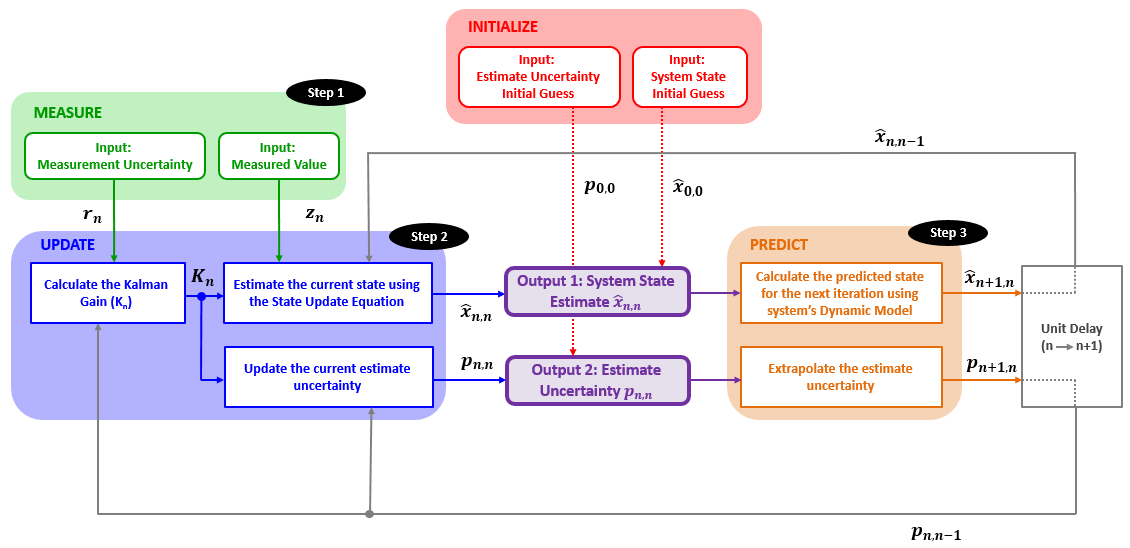
\includegraphics[scale=0.45]{imgs/DetailedKalmanFilterAlgorithm.png}
    \caption{卡尔曼滤波器框图}
    \label{fig:KalmanFilter}
\end{figure}

\subsection{非线性模型的近似原理}
对于线性卡尔曼滤波器,当系统为线性高斯模型时,滤波器能给出最优的估计,但是实际系统总是存在不同程度的非线性,如平方、三角关系、开方等。对于非线性系统,可以采用的一种方法是通过线性化方法将非线性系统转换为近似的线性系统,即为扩展卡尔曼滤波,核心思想是:围绕滤波值将非线性函数展开成泰勒级数并略去二阶及以上项,得到一个近似的线性化模型\cite{julier2004unscented},然后应用卡尔曼滤波完成状态估计。扩展卡尔曼滤波算法的详细推导过程\cite{CKF}如下:

在扩展卡尔曼滤波中,状态转换和观测模型不再需要是状态的线性函数,而可以是\textbf{可微函数}。这里${w}_{k}$和${v}_{k}$是过程噪声和观测噪声,它们都假定为零均值多元高斯噪声,分别具有协方差$\mathbf{Q_k}$和$\mathbf{R_k}$。$\mathbf{u_k}$ 是控制向量。
\begin{equation*}
\begin{array}{l}
\mathbf{x}_{k}=f\left(\mathbf{x}_{k-1}, \mathbf{u}_{k}\right)+\mathbf{w}_{k} \\
\mathbf{z}_{k}=h\left(\mathbf{x}_{k}\right)+\mathbf{v}_{k}
\end{array}
\end{equation*}

在扩展卡尔曼滤波中,状态的预测以及观测值的预测由非线性函数计算得出,线性卡尔曼滤波中的状态转移矩阵和观测矩阵由$f$和$h$函数的\textbf{雅克比矩阵}代替,即

\begin{equation*}
f_{k}=\left.\frac{\partial f}{\partial \mathbf{x}_{k}}\right|_{\mathbf{x}_{k}=\mathbf{\hat x}_{k \mid k}}\quad
h_{k} = \left.\frac{\partial h}{\partial \mathbf{x}_{k}}\right|_{\mathbf{x}_{k}=\mathbf{\hat x}_{k \mid k}}
\end{equation*}

假设我们已知$k$时刻状态估计值$\mathbf{\hat x}_{k \mid k}$和估计方差$\mathbf{P}_{k \mid k}$,我们将非线性函数$f\left(\mathbf{x}_{k}\right)$在$\mathbf{\hat x}_{k \mid k}$ 处进行一阶泰勒展开可得:

\begin{equation*}
    f\left(\mathbf{x}_{k}\right)=f\left(\mathbf{\hat x}_{k \mid k}\right)+\left.\frac{\partial f}{\partial \mathbf{x}_{k}}\right|_{\mathbf{x}_{k}=\mathbf{\hat x}_{k \mid k}}\left(\mathbf{x}_{k}-\mathbf{\hat x}_{k \mid k}\right)+o\left(\mathbf{x}_{k}-\mathbf{\hat x}_{k \mid k}\right)
\end{equation*}

其中$o\left(\mathbf{x}_{k}-\mathbf{\hat x}_{k \mid k}\right)$为高阶项。

忽略高阶项, 状态方程可以化简为: 

\begin{equation*}
    \mathbf{x}_{k+1}=f\left(\mathbf{\hat x}_{k \mid k}\right)+f_{k}\left(\mathbf{x}_{k}-\mathbf{\hat x}_{k \mid k}\right)+\mathbf{w}_{k} 
\end{equation*}

一步状态预测:
\begin{equation*}
    \mathbf{\hat x}_{k+1 \mid k}=\mathrm{E}\left[f\left(\mathbf{\hat x}_{k \mid k}\right)+f_{k}\left(\mathbf{x}_{k}-\mathbf{\hat x}_{k \mid k}\right)+\mathbf{w}_{k}\right]=f\left(\mathbf{\hat x}_{k \mid k}\right)
\end{equation*}

一步预测协方差:
\begin{equation*}
\begin{aligned}
\mathbf{P}_{k+1 \mid k} &=\mathrm{E}\left[\left(\mathbf{x}_{k+1}-\mathbf{\hat x}_{k+1 \mid k}\right)\left(\mathbf{x}_{k+1}-\mathbf{\hat x}_{k+1 \mid k}\right)^{\mathbf{T}}\right] \\
&=\mathrm{E}\left\{\left[f_{k}\left(\mathbf{x}_{k}-\mathbf{\hat x}_{k \mid k}\right)+\mathbf{w}_{k}\right]\left[f_{k}\left(\mathbf{x}_{k}-\mathbf{\hat x}_{k \mid k}\right)+\mathbf{w}_{k}\right]^{\mathbf{T}}\right\} \\
&=f_{k} \mathbf{P}_{k \mid k} f_{k}^{\mathbf{T}}+\mathbf{Q}_{k}
\end{aligned}
\end{equation*}

将非线性函数$h(\cdot)$在一步状态预测$\hat{\mathbf{x}}_{k+1 \mid k}$  处一阶泰勒展开得:
\begin{equation*}
h\left(\mathbf{x}_{k+1}\right)=h\left(\mathbf{\hat x}_{k+1 \mid k}\right)+\left.\frac{\partial h}{\partial \mathbf{x}_{k+1}}\right|_{\mathbf{x}_{k+1}=\mathbf{\hat x}_{k+1 k}}\left(\mathbf{x}_{k+1}-\mathbf{\hat x}_{k+1 \mid k}\right)+o\left(\mathbf{x}_{k+1}-\mathbf{\hat x}_{k+1 \mid k}\right)
\end{equation*}

其中$o\left(\mathbf{x}_{k+1}-\mathbf{\hat x}_{k+1 \mid k}\right)$为高阶项, 所以量测方程可表示为: 
\begin{equation*}
    \mathbf{z}_{k+1}=h\left(\hat{\mathbf{x}}_{k+1 \mid k}\right)+h_{k+1}\left(\mathbf{x}_{k+1}-\hat{\mathbf{x}}_{k+1 \mid k}\right)+\mathbf{v}_{k+1} 
\end{equation*}

所以量测一步预测:
\begin{equation*}
    \mathbf{\hat z}_{k+1}=\mathrm{E}\left[h\left(\hat{\mathbf{x}}_{k+1 \mid k}\right)+h_{k+1}\left(\mathbf{x}_{k+1}-\hat{\mathbf{x}}_{k+1 \mid k}\right)+\mathbf{v}_{k+1}\right]=h\left(\hat{\mathbf{x}}_{k+1 \mid k}\right)
\end{equation*}


量测预测误差协方差阵:
\begin{equation*}
    \begin{aligned}
    \mathbf{P}_{z z, k+1 \mid k} &=\mathrm{E}\left[\left(\mathbf{z}_{k+1}-\mathbf{\hat z}_{k+1}\right)\left(\mathbf{z}_{k+1}-\mathbf{\hat z}_{k+1}\right)^{\mathbf{T}}\right] \\
    &=\mathrm{E}\left\{\left[h_{k+1}\left(\mathbf{x}_{k+1}-\hat{\mathbf{x}}_{k+1 \mid k}\right)+\mathbf{v}_{k+1}\right]\left[h_{k+1}\left(\mathbf{x}_{k+1}-\hat{\mathbf{x}}_{k+1 \mid k}\right)+\mathbf{v}_{k+1}\right]^{\mathbf{T}}\right\} \\
    &=h_{k+1} \mathbf{P}_{k+1 \mid k} h_{k+1}^{\mathbf{T}}+\mathbf{R}_{k+1}
    \end{aligned}
\end{equation*}

状态与量测间的互协方差矩阵:
\begin{equation*}
    \begin{aligned}
    \mathbf{P}_{x z, k+1 \mid k} &=\mathrm{E}\left[\left(\mathbf{x}_{k+1}-\hat{\mathbf{x}}_{k+1}\right)\left(\mathbf{z}_{k+1}-\hat{\mathbf{z}}_{k+1}\right)^{\mathbf{T}}\right] \\
    &=\mathrm{E}\left\{\left(\mathbf{x}_{k+1}-\hat{\mathbf{x}}_{k+1}\right)\left[h_{k+1}\left(\mathbf{x}_{k+1}-\hat{\mathbf{x}}_{k+1 \mid k}\right)+\mathbf{v}_{k+1}\right]^{\mathbf{T}}\right\} \\
    &=\mathbf{P}_{k+1 \mid k} h_{k+1}^{\mathbf{T}}
    \end{aligned}
\end{equation*}

状态增益矩阵:
\begin{equation*}
    \mathbf{K}_{k+1}=\mathbf{P}_{x z, k+1 \mid k}\left(\mathbf{P}_{z z, k+1 \mid k}\right)^{-1}=\mathbf{P}_{k+1 \mid k} h_{k+1}^{\mathbf{T}}\left(h_{k+1} \mathbf{P}_{k+1 \mid k} h_{k+1}^{\mathbf{T}}+\mathbf{R}_{k+1}\right)^{-1}
\end{equation*}
     
 k+1时刻状态估计值: 
 \begin{equation*}
     \mathbf{\hat x}_{k+1 \mid k+1}=\mathbf{\hat x}_{k+1 \mid k}+\mathbf{K}_{k+1}\left(\mathbf{z}_{k+1}-\hat{\mathbf{z}}_{k+1 \mid k}\right)
 \end{equation*}


状态估计误差协方差矩阵:
\begin{equation*}
    \begin{aligned}
    \mathbf{P}_{k+1 \mid k+1} &=\mathrm{E}\left[\left(\mathbf{x}_{k+1}-\mathbf{\hat x}_{k+1 \mid k+1}\right)\left(\mathbf{x}_{k+1}-\mathbf{\hat x}_{k+1 \mid k+1}\right)^{\mathbf{T}}\right] \\
    &=\mathrm{E}\left\{\left[\mathbf{x}_{k+1}-\mathbf{\hat x}_{k+1 k}-\mathbf{K}_{k+1}\left(\mathbf{z}_{k+1}-\hat{\mathbf{z}}_{k+1 \mid k}\right)\right]\left[\mathbf{x}_{k+1}-\mathbf{\hat x}_{k+1 \mid k}-\mathbf{K}_{k+1}\left(\mathbf{z}_{k+1}-\hat{\mathbf{z}}_{k+1 k}\right)\right]^{\mathbf{T}}\right\} \\
    &=\left(\mathbf{I}-\mathbf{K}_{k+1} h_{k+1}\right) \mathbf{P}_{k+1 k}\left(\mathbf{I}-\mathbf{K}_{k+1} h_{k+1}\right)^{T}+\mathbf{K}_{k+1} \mathbf{R}_{k+1} \mathbf{K}_{k+1}^{T} \\
    &=\left(\mathbf{I}-\mathbf{K}_{k+1} h_{k+1}\right) \mathbf{P}_{k+1 k}
    \end{aligned}f
\end{equation*}

于是就可以归纳出EKF的公式。
预测方程:
\begin{equation*}
    \begin{array}{l}
    \hat{\mathbf{x}}_{k \mid k-1}=f\left(\hat{\mathbf{x}}_{k-1 \mid k-1}, \mathbf{u}_{k}\right) \\
    \mathbf{P}_{k \mid k-1}=f_{k} \mathbf{P}_{k-1 \mid k-1} f_{k}^{\top}+\mathbf{Q}_{k} 
    \end{array}
\end{equation*}

更新方程:
\begin{equation*}
\begin{array}{l}
\tilde{\mathbf{y}}_{k}=\mathbf{z}_{k}-h\left(\hat{\mathbf{x}}_{k \mid k-1}\right)\\
\mathbf{S}_{k}=h_{k} \mathbf{P}_{k \mid k-1} h_{k}^{\top}+\mathbf{R}_{k} \\
\mathbf{K}_{k}=\mathbf{P}_{k \mid k-1} h_{k}^{\top} \mathbf{S}_{k}^{-1} \\
\hat{\mathbf{x}}_{k \mid k}=\hat{\mathbf{x}}_{k \mid k-1}+\mathbf{K}_{k} \tilde{\mathbf{y}}_{k} \\
\mathbf{P}_{k \mid k}=\left(\mathbf{\mathbf{I}}-\mathbf{K}_{k} h_{k}\right) \mathbf{P}_{k \mid k-1}
\end{array}
\end{equation*}

\section{扩展卡尔曼滤波的算法}
\subsection{流程及参数}
扩展卡尔曼滤波算法的流程与卡尔曼滤波基本相同,大致可以总结为流程图\ref{fig:EKFflow}:其中需要使用者设置的参数,除了要通过具体模型确定\textbf{状态转移方程}和确定\textbf{观测方程}之外,主要有:
\begin{itemize}
    \item 初始的状态变量$\mathbf{x}_{0}$
    \item $\mathbf{x}_{0}$的协方差$\mathbf{P}_{0}$
    \item 状态转移矩阵$\mathbf{A}$
    \item 过程激励噪声协方差$\mathbf{Q}$
    \item 测量噪声协方差$\mathbf{R}$
\end{itemize}

\subsection{MATLAB中扩展卡尔曼滤波的函数的用法}
我在Matlab找到了extendedKalmanFilter和trackingEKF两个类,发现在使用时基本上可以相互替换,查阅源码发现它们都继承自matlabshared.tracking.internal.ExtendedKalmanFilter这个超类。因此无论是参数还是用法都基本上一致。
\subsubsection{extendedKalmanFilter}
obj = extendedKalmanFilter(StateTransitionFcn,MeasurementFcn,InitialState) 创建一个扩展的卡尔曼滤波对象,用于离散时间非线性系统的在线状态估计。 StateTransitionFcn 是一个函数,它计算系统在时间 $k-1$ 的状态向量下的时间 $k$。 MeasurementFcn是一个函数,它计算系统在时间 $k$ 的输出测量值,给定时间 $k$ 的状态。 InitialState指定状态估计值的初始值。

创建对象后,使用 correct 和 predict 命令,使用一阶离散时间扩展卡尔曼滤波算法和实时数据来更新状态估计值和状态估计误差协方差值。

还有一些可选属性可以设置:通过State设置初始状态,通过StateCovariance设置初始状态的协方差,通过ProcessNoise设置过程激励噪声协方差,通过MeasurementNoise设置测量噪声协方差。

\subsubsection{trackingEKF}
参数和前者完全一致。区别在于提供了预定义的状态更新和测量函数。在本次课设中我们将自定义状态更新和测量函数。


%\begin{itemize}
%item[1] \textbf{初始化}
%$$
%hat{\mathbf{x}}_{0 \mid 0}=\mathrm{E}(\mathbf{x}_0),\quad
%mathbf{P}_{0 \mid 0} = \mathrm{Cov}(\mathbf{x}_0)
%$$
%\item[2] \textbf{时间更新(预测)}

%\item[3] \textbf{测量更新(校正)}

%\item[4] \textbf{回到第二步继续循环}
%\end{itemize}


\begin{figure}
    \centering
    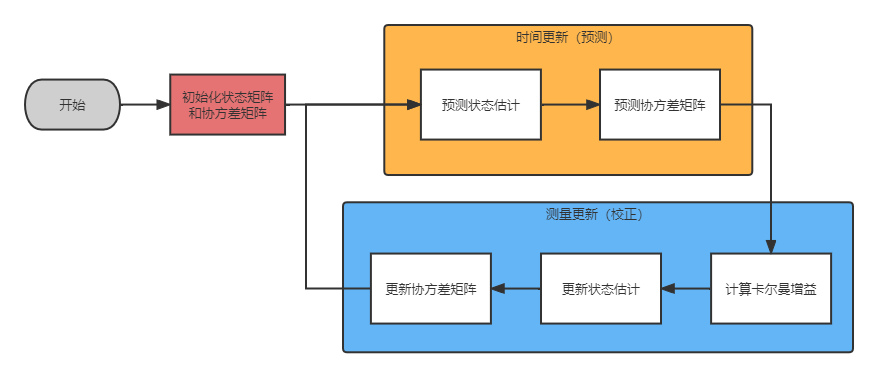
\includegraphics[width = 0.9\textwidth]{imgs/EKF.png}
    \caption{扩展卡尔曼滤波流程图}
    \label{fig:EKFflow}
\end{figure}

\section{目标跟踪系统的模型}
时刻$n$的状态向量为
\begin{equation}
    \mathbf{s}[n]=\left[\begin{array}{l}
    r_{x}[n] \\
    r_{y}[n] \\
    v_{x}[n] \\
    v_{y}[n]
    \end{array}\right]
\end{equation}


状态向量的四个分量的物理意义分别为:运动目标在时刻$n$的横轴位置、纵轴位置、横轴速度与纵轴速度。假定时刻$n=0$为初始时刻,$n=1$为首次观测的时刻, $T$为采样间隔。状态转移方程的标量形式为:

\begin{equation}
\begin{array}{l}
    r_{x}[n]=r_{x}[n-1]+v_{x}[n-1] T,\\
    r_{y}[n]=r_{y}[n-1]+v_{y}[n-1] T.
\end{array}
\end{equation}
\begin{equation}
\begin{array}{l}
    v_{x}[n]=v_{x}[n-1]+u_{x}[n],\\
    v_{y}[n]=v_{y}[n-1]+u_{y}[n].
\end{array}
\end{equation}

过程噪声$u_{x}[n]$与$u_{y}[n]$的物理意义是随机加速度。$u_{x}[n]$与$u_{y}[n]$独立同分布, 均服从均值为0, 方差为$\sigma_{u}^{2}$的正态分布。
观测方程的标量形式为
\begin{equation}
    \hat{R}[n]=\sqrt{r_{x}^{2}[n]+r_{y}^{2}[n]}+w_{R}[n],
\end{equation}
\begin{equation}
    \hat{\beta}[n]=\arctan \frac{r_{y}[n]}{r_{x}[n]}+w_{\beta}[n] .
\end{equation}

第一个观测分量的物理意义是目标到原点的距离;第二个观测分量的物理意义是目标到原点的连线与 横轴的夹角。观测噪声$w_{R}[n] $与$w_{\beta}[n]$相互独立, 且均服从均值为 0 的正态分布; 前者的方差为$\sigma_{R}^{2}$, 后 者的方差为$\sigma_{\beta}^{2}$。注意,$ \hat{\beta}[n]$的单位是弧度。
我们记
$$
\hat{\mathbf{C}}[n]=\left[\begin{array}{cc}
\sigma_{R}^{2} & 0 \\
0 & \sigma_{\beta}^{2}
\end{array}\right]
$$
 利用一阶泰勒级数展开把非线性问题变为线性问题得到如下公式:
 预测: 
 \begin{equation}
    \hat{\mathbf{s}}[n \mid n-1]=\mathbf{A} \hat{\mathbf{s}}[n-1 \mid n-1]
 \end{equation}
 
最小预测 MSE 矩阵:
\begin{equation}
    \mathbf{M}[n \mid n-1]=\mathbf{A} \mathbf{M}[n-1 \mid n-1] \mathbf{A}^{T}+\mathbf{Q} 
\end{equation}

卡尔曼增益矩阵:
\begin{equation}
     \mathbf{K}[n]=\mathbf{M}\left[n \mid n-1 \right] h^{T}[n] 
 \left(\mathbf{C}[n]+h[n] \mathbf{M}[n \mid n-1] h^{T}[n]\right)^{-1} 
\end{equation}

校正:
\begin{equation}
    \hat{\mathbf{s}}[n \mid n] =\hat{\mathbf{s}}[n \mid n-1]+\mathbf{K}[n]    (\mathbf{Z}[n]-h(\mathbf{s}[n \mid n-1]))
\end{equation}

最小MSE矩阵:
\begin{equation}
    \mathbf{M}[n \mid n]=(\mathbf{I}-\mathbf{K}[n] h[n]) \mathbf{M}[n \mid n-1]
\end{equation}

由(1-3)可知:
\begin{equation}
    \mathbf{s}[n]=\left[\begin{array}{llll}
    1 & 0 & T & 0 \\
    0 & 1 & 0 & T \\
    0 & 0 & 1 & 0 \\
    0 & 0 & 0 & 1
    \end{array}\right]
    \mathbf{s}[n-1]+\left[\begin{array}{c}
    0 \\
    0 \\
    u_{x}[n] \\
    u_{y}[n]
    \end{array}\right]
\end{equation}

因此,状态转移矩阵$\mathbf{A}$和过程激励噪声协方差矩阵$\mathbf{Q}$如下
\begin{equation}
    \mathbf{A}=\left[\begin{array}{llll}
    1 & 0 & T & 0 \\
    0 & 1 & 0 & T \\
    0 & 0 & 1 & 0 \\
    0 & 0 & 0 & 1
    \end{array}\right], \mathbf{Q}=\left[\begin{array}{cccc}
    0 & 0 & 0 & 0 \\
    0 & 0 & 0 & 0 \\
    0 & 0 & \sigma_{u}^{2} & 0 \\
    0 & 0 & 0 & \sigma_{u}^{2}
    \end{array}\right]
\end{equation}

$h$的雅可比矩阵就为:
\begin{equation}
    \mathbf{H}[n]=\left.\frac{\partial \hat{h}}{\partial \mathbf{s}[n]}\right|_{\mathbf{s}[n]=\mathbf{\hat{s}}[n \mid n-1]} 
    =\left[\begin{array}{llll}
    \frac{r_{x}[n]}{\sqrt{r_{x}^{2}[n]+r_{y}^{2}[n]}} & \frac{r_{y}[n]}{\sqrt{r_{x}^{2}[n]+r_{y}^{2}[n]}} & 0 & 0\\
    \frac{-r_{y}[n]}{r_{x}^{2}[n]+r_{y}^{2}[n]} & \frac{r_{x}[n]}{r_{x}^{2}[n]+r_{y}^{2}[n]} & 0 & 0\\
    \end{array}\right]
\end{equation}

\section{仿真实验结果}
\subsection{基本要求}
仿真实验结果如图[3-11]所示。
由图[6-9]可见,EKF估计所得的$r_x,r_y,u_x,u_y$和状态方程决定的较为接近,但是EKF估计所得的$\hat{r}_y$变化更平缓。

我们观察图\ref{fig:chart7}可以看到预测轨迹和真实轨迹基本一致
再根据图\ref{fig:chart8}可以看到预测的误差值基本维持在0.4m以下。
\begin{figure}
    \centering
    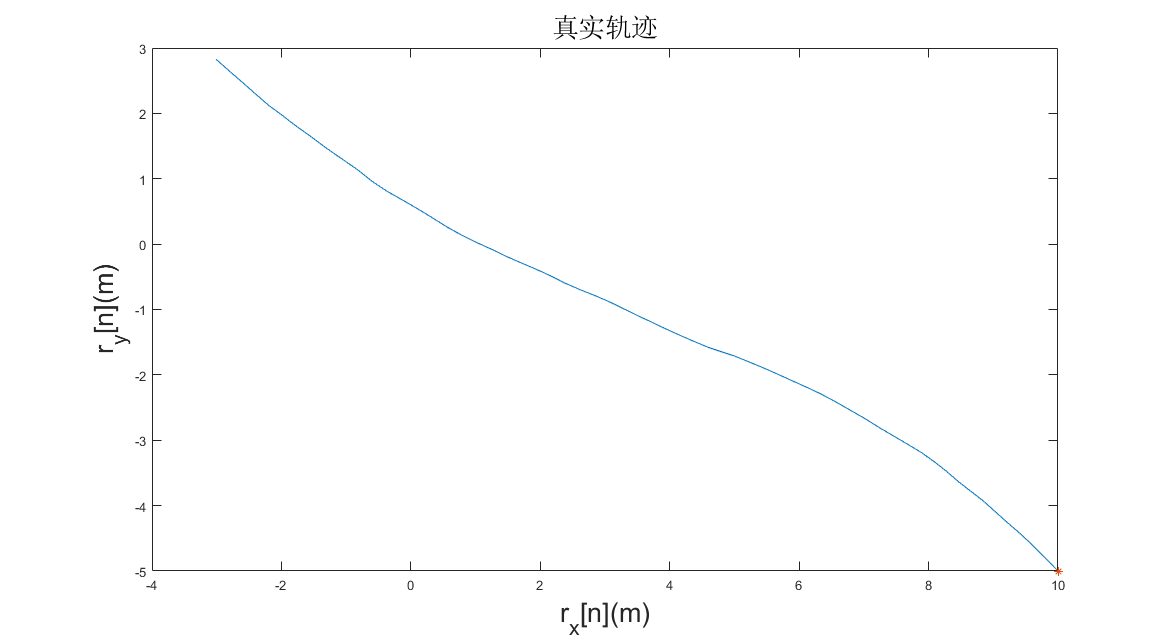
\includegraphics[width = 0.9\textwidth]{imgs/1.png}
    \caption{$r_x[n]-r_y[n]$}
    \label{fig:chart1}
\end{figure}
\begin{figure}
    \centering
    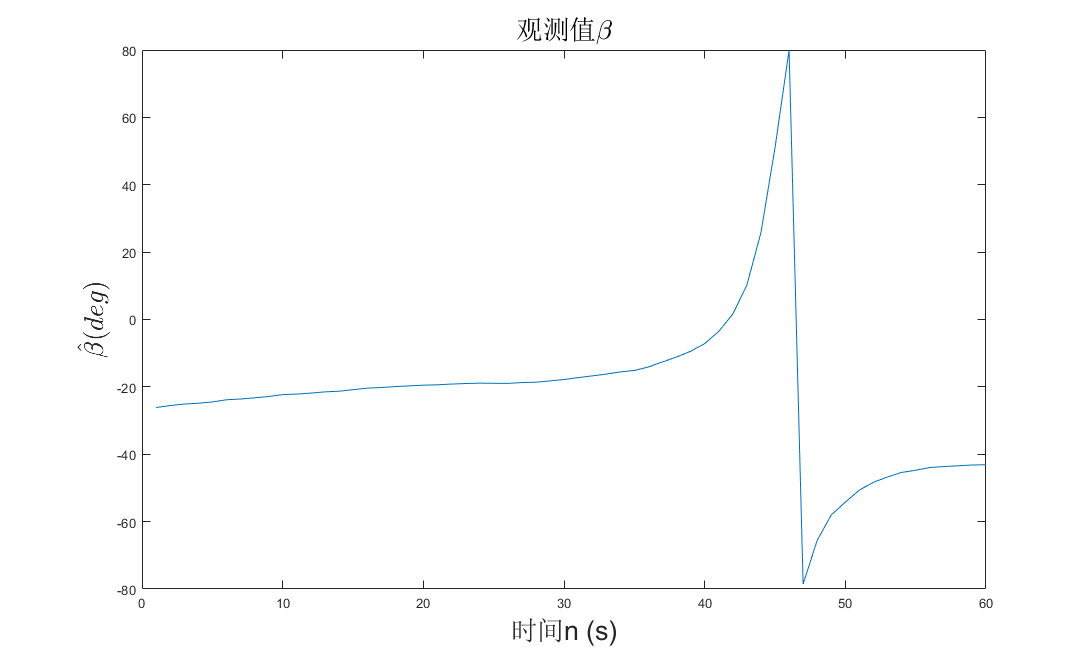
\includegraphics[width = 0.9\textwidth]{imgs/2.png}
    \caption{$n-\hat{R}[n]$}
    \label{fig:chart2}
\end{figure}
\begin{figure}
    \centering
    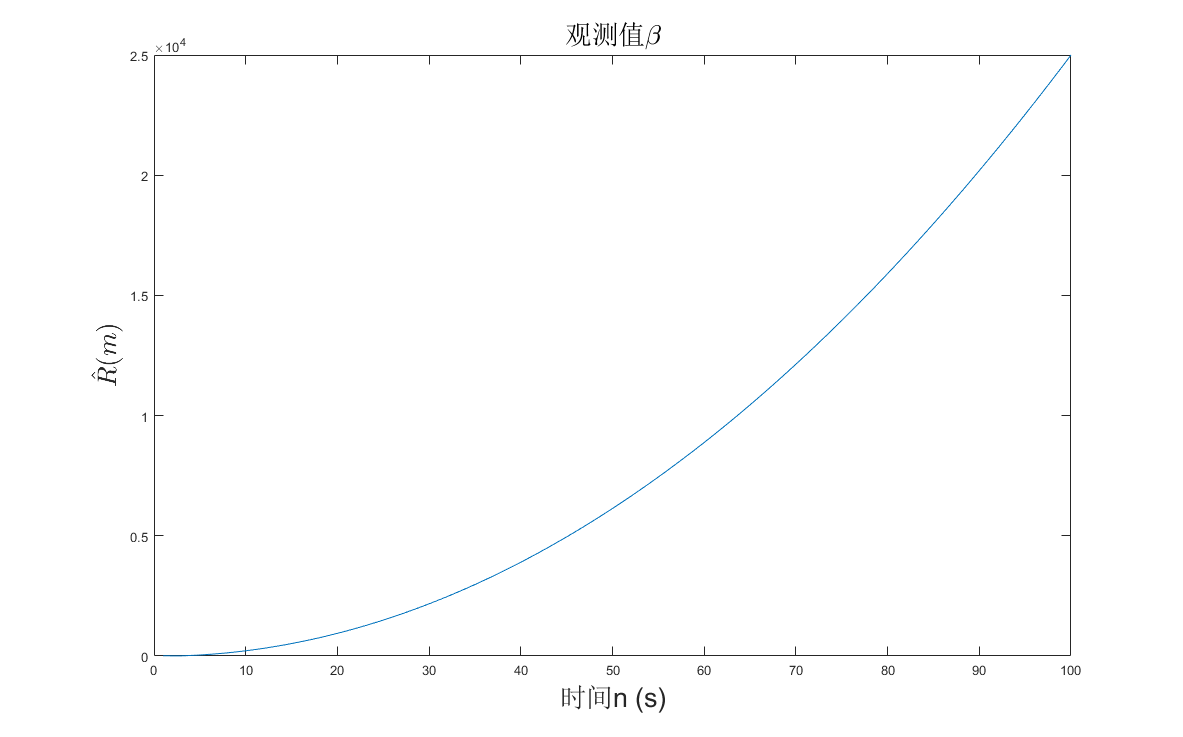
\includegraphics[width = \textwidth]{imgs/3.png}
    \caption{$n-\hat{\beta}[n]$}
    \label{fig:chart3}
\end{figure}
\begin{figure}
    \centering
    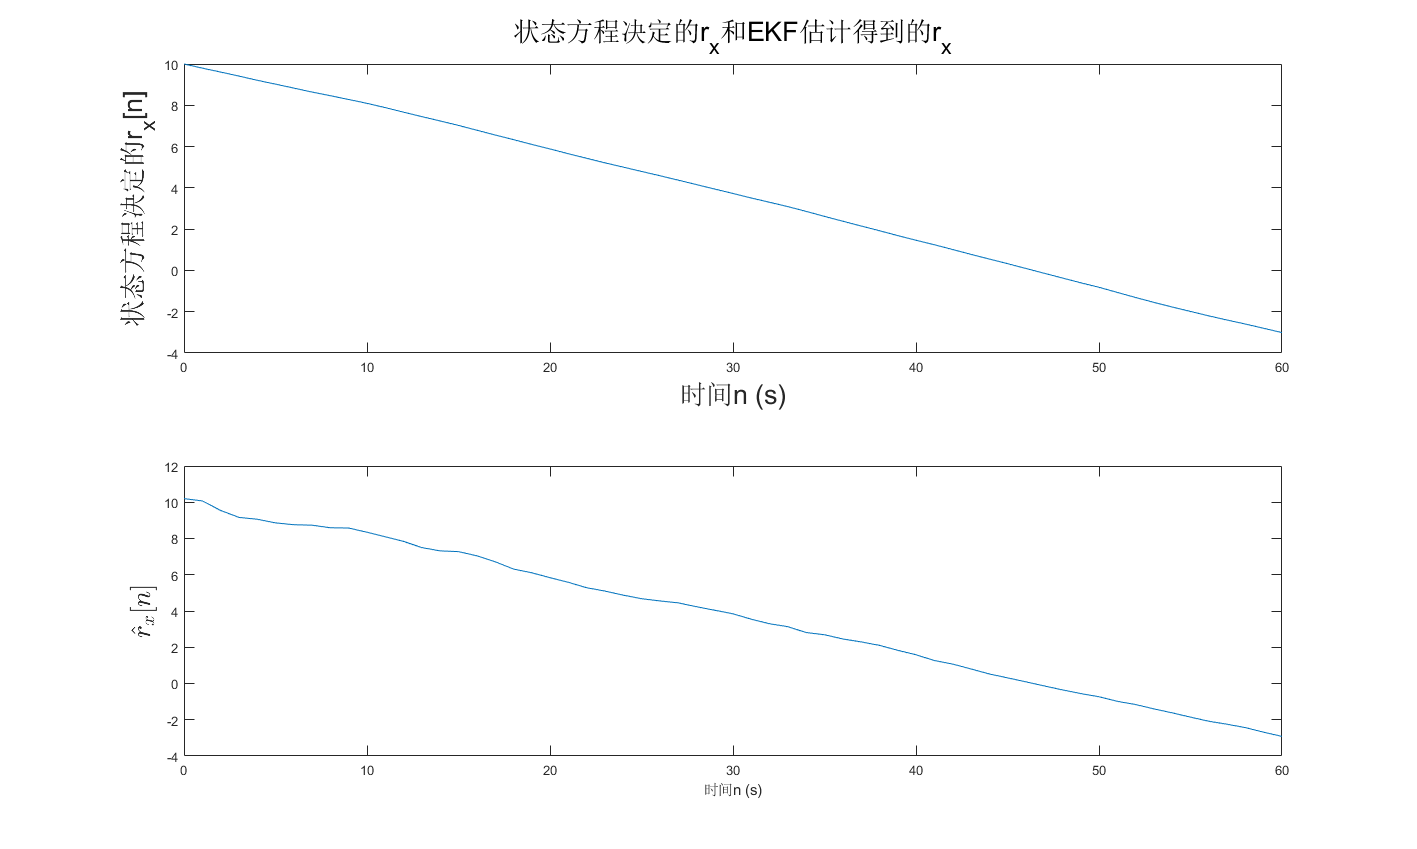
\includegraphics[width = \textwidth]{imgs/4.png}
    \caption{$r_x[n]-\hat{r}_x[n]$}
    \label{fig:chart4}
\end{figure}
\begin{figure}
    \centering
    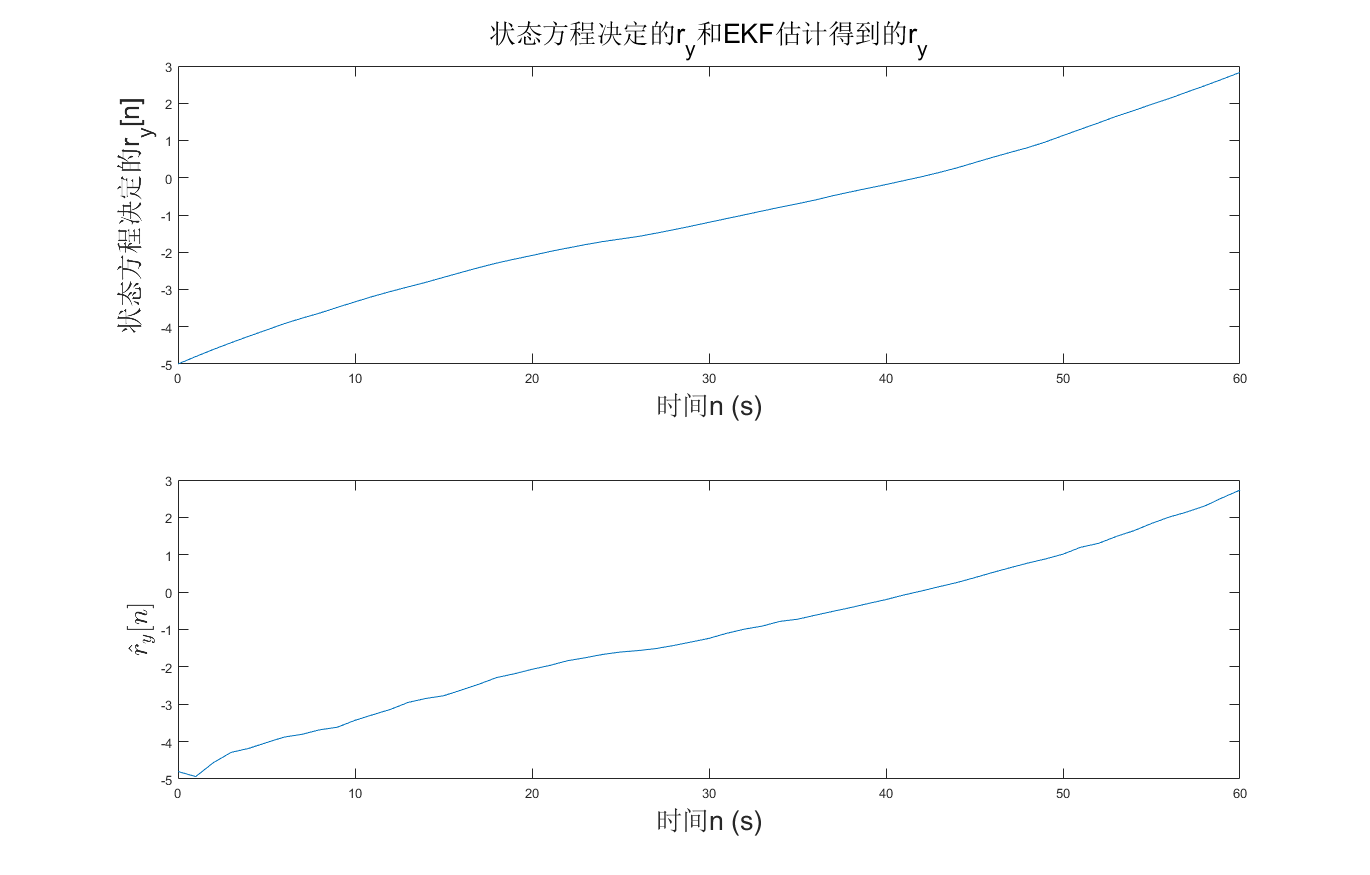
\includegraphics[width = \textwidth]{imgs/5.png}
    \caption{$r_y[n]-\hat{r}_y[n]$}
    \label{fig:chart5}
\end{figure}
\begin{figure}
    \centering
    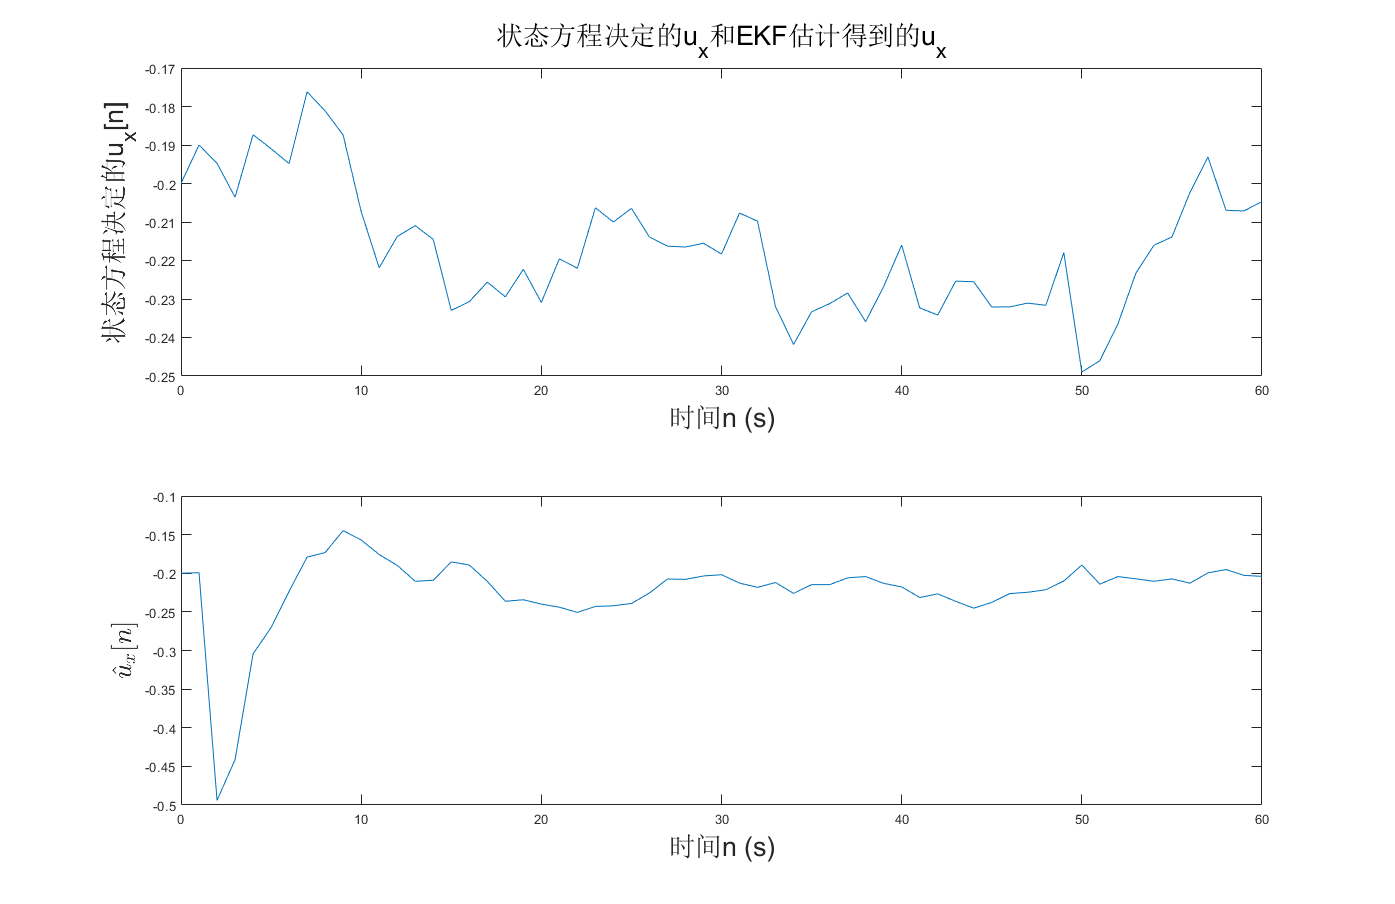
\includegraphics[width = \textwidth]{imgs/6.png}
    \caption{$u_x[n]-\hat{u}_x[n]$}
    \label{fig:chart6}
\end{figure}
\begin{figure}
    \centering
    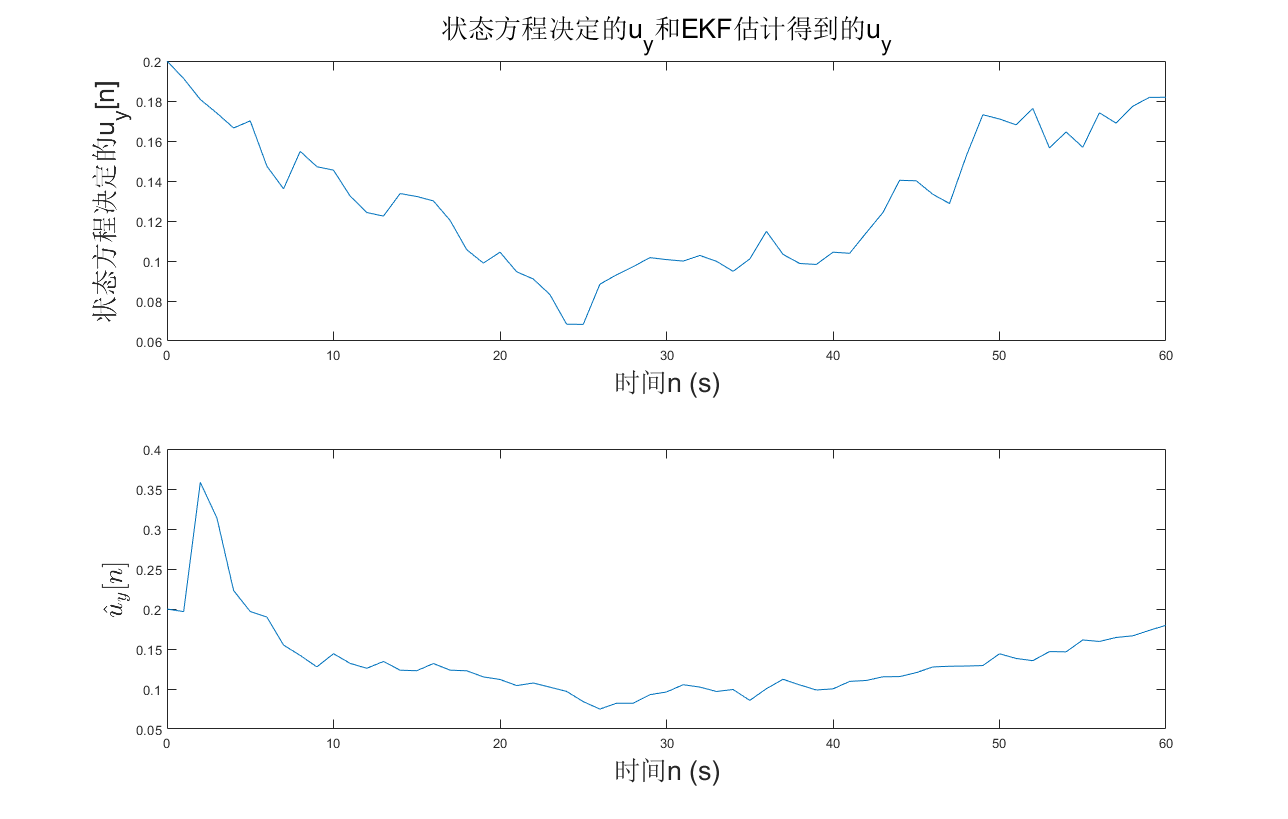
\includegraphics[width = \textwidth]{imgs/7.png}
    \caption{$u_y[n]-\hat{u}_y[n]$}
    \label{fig:chart7}
\end{figure}

\begin{figure}
    \centering
    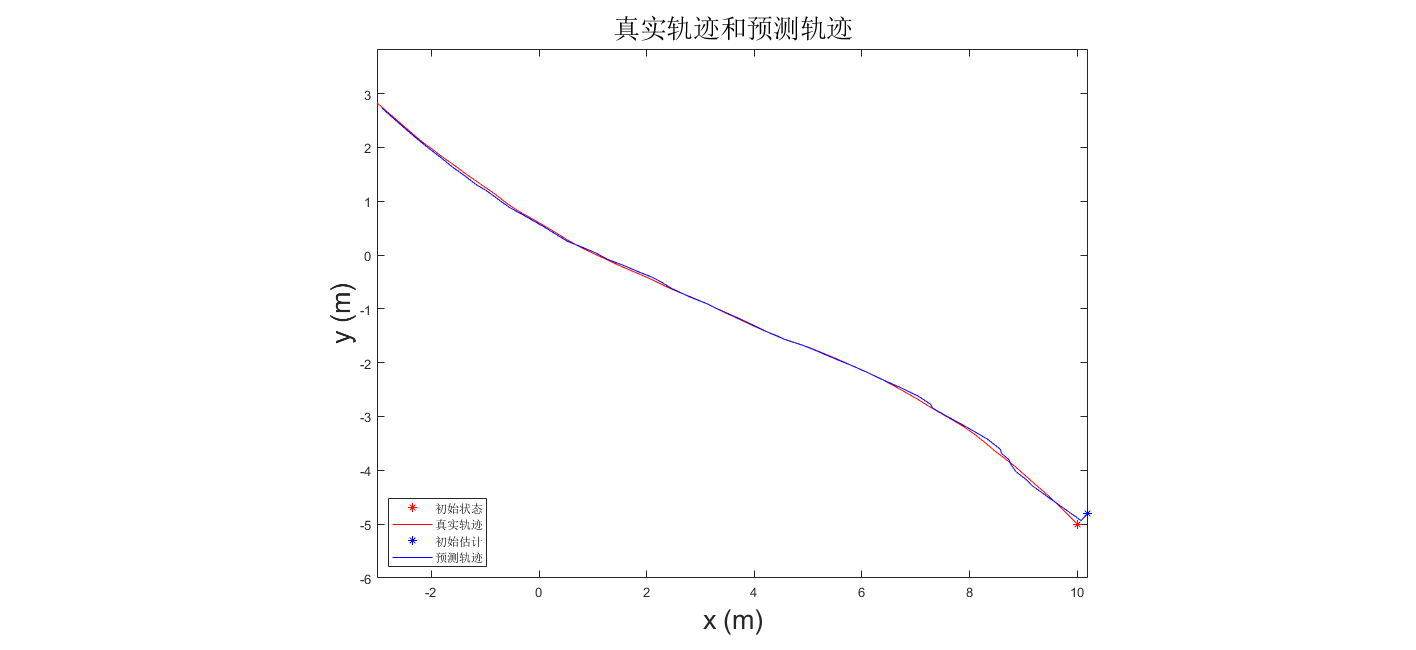
\includegraphics[width = \textwidth]{imgs/8.png}
    \caption{真实轨迹和预测轨迹}
    \label{fig:chart8}
\end{figure}

\begin{figure}
    \centering
    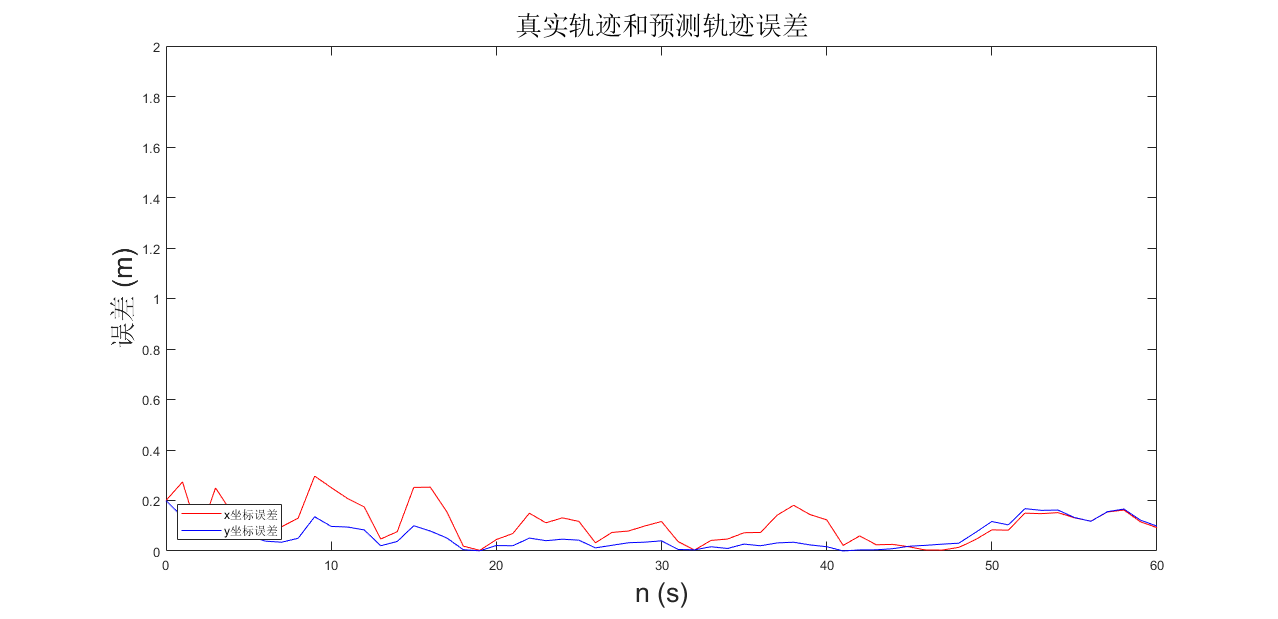
\includegraphics[width =0.9\textwidth]{imgs/9.png}
    \caption{误差}
    \label{fig:chart9}
\end{figure}

\subsection{敏感性分析}
我们改变$\mathbf{x}_0$:改变初始位置$r_x[0],r_y[0]$发现除了在初期影响比较大之外,后来都会收敛成相似的曲线。所以猜测EKF对$r_x[0],r_y[0]$并不敏感。改变变初始速度$u_x[0],u_y[0]$,发现当初始速度误差太大时,无法准确预测路径。猜测EKF对$u_x[0],u_y[0]$较为敏感。
\begin{figure}[ht]
    \centering
    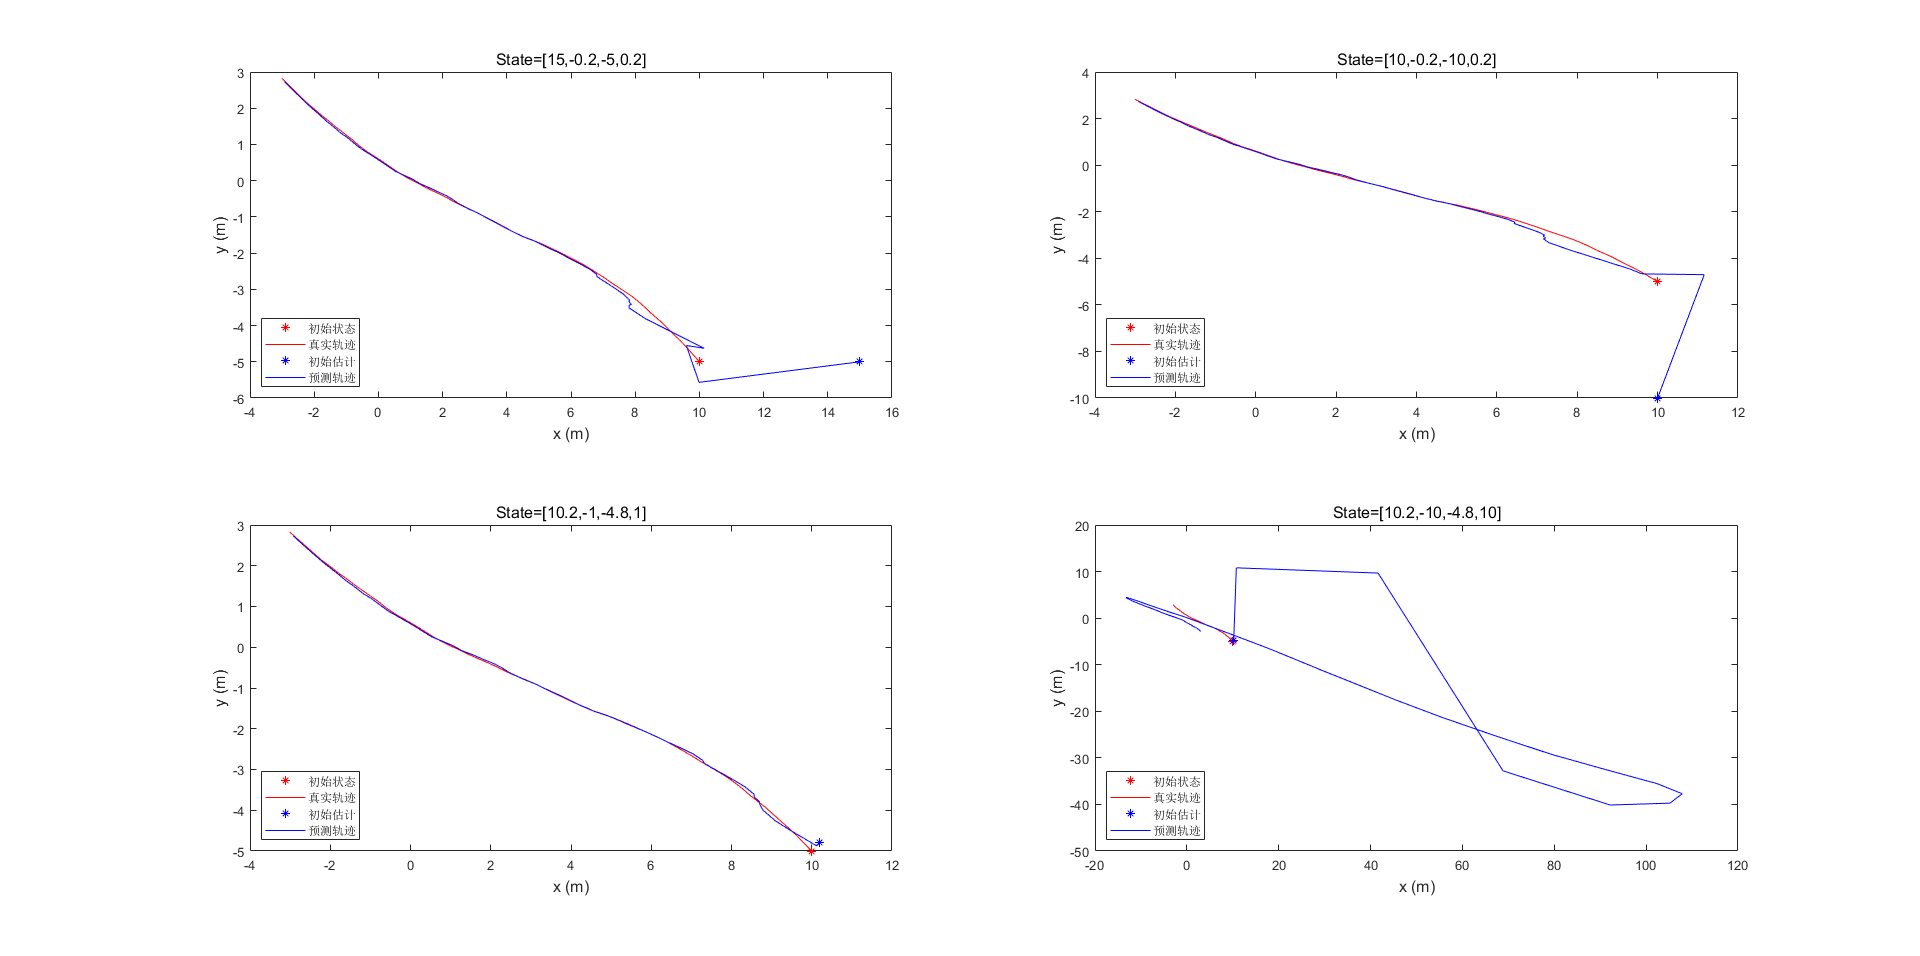
\includegraphics[width = \textwidth]{imgs/comp1.png}
    \caption{改变$\mathbf{x}_0$}
    \label{fig:comp1}
\end{figure}

我们改变$\mathbf{P}_0$发现都会收敛成相似的曲线。所以猜测EKF对$\mathbf{P}_0$并不敏感。
\begin{figure}[ht]
    \centering
    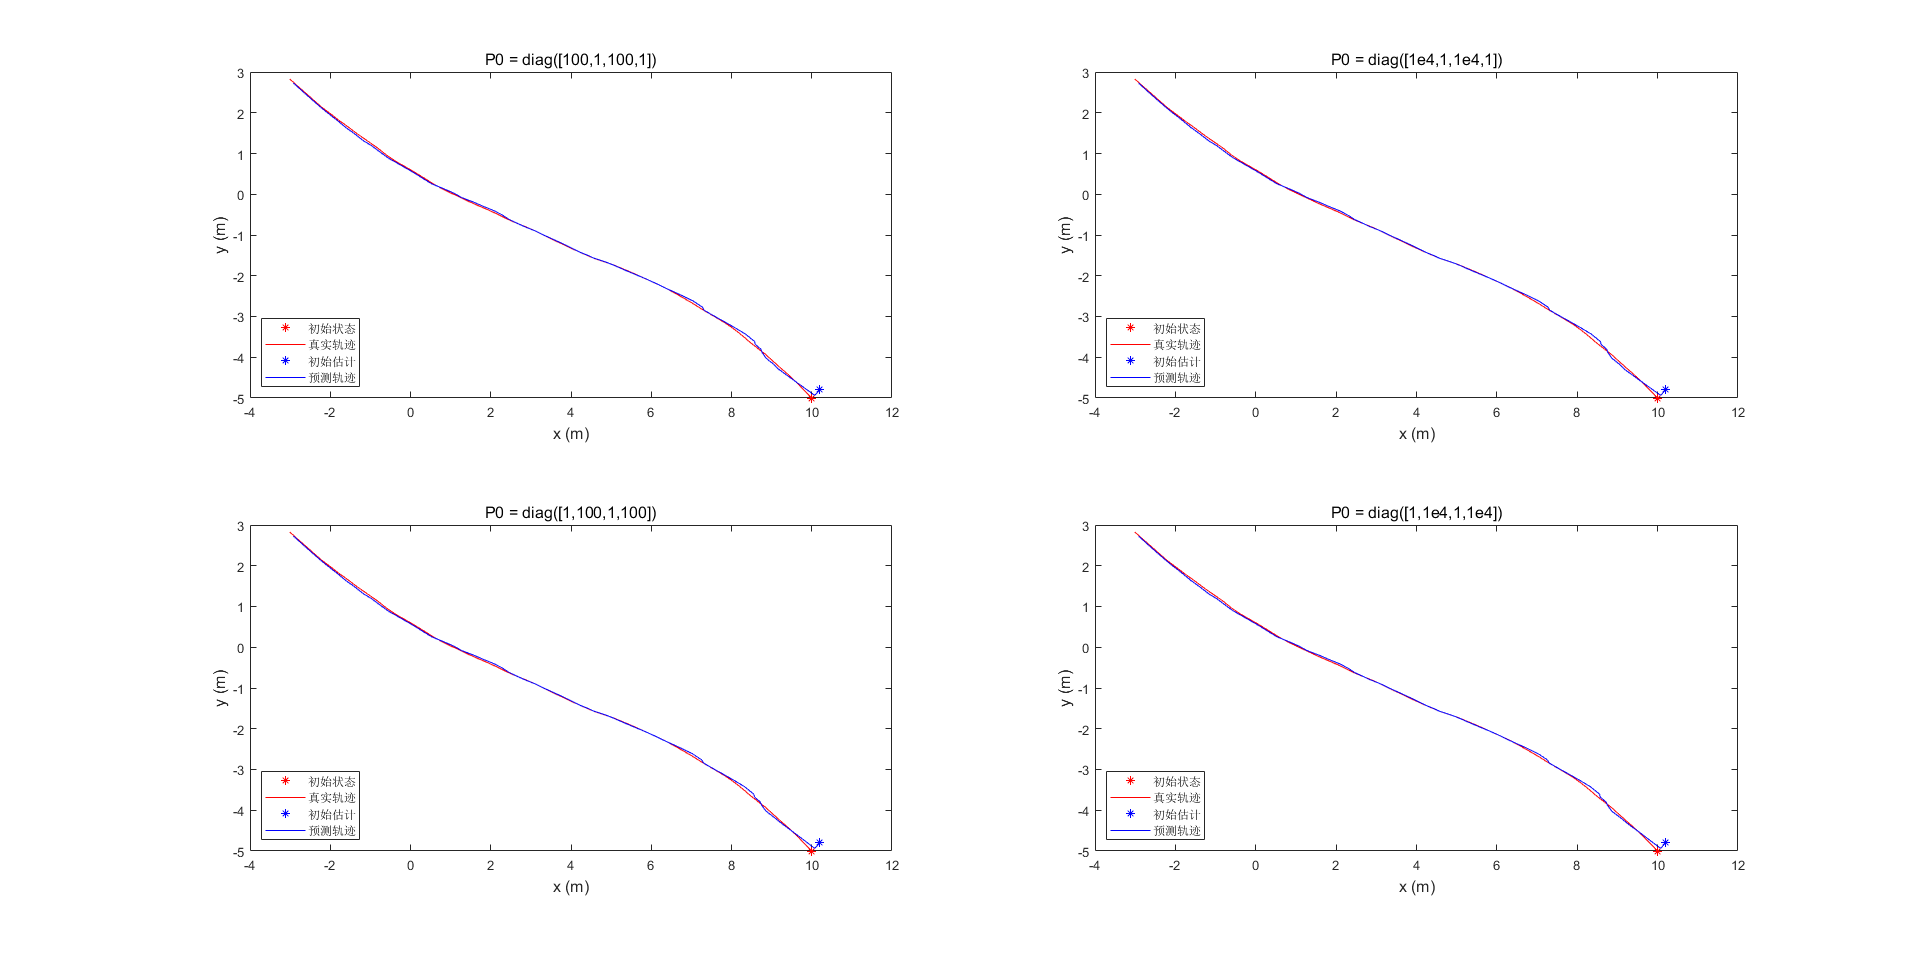
\includegraphics[width = 0.9\textwidth]{imgs/comp2.png}
    \caption{改变$\mathbf{P}_0$}
    \label{fig:comp2}
\end{figure}

综上所述,设置良好的初始位置有利于预测曲线在短时间内达到比较好的精确程度,但是在时间较长的情况下,对于长期的精确程度影响不大。初始状态的速度则比较重要,如果误差过大则无法预测。协方差矩阵影响不大。

我们改变过程激励噪声协方差$\mathbf{Q}$,发现当其过小时,会导致预测曲线过于超前,太大则会导致无法预测。
\begin{figure}[H]
    \centering
    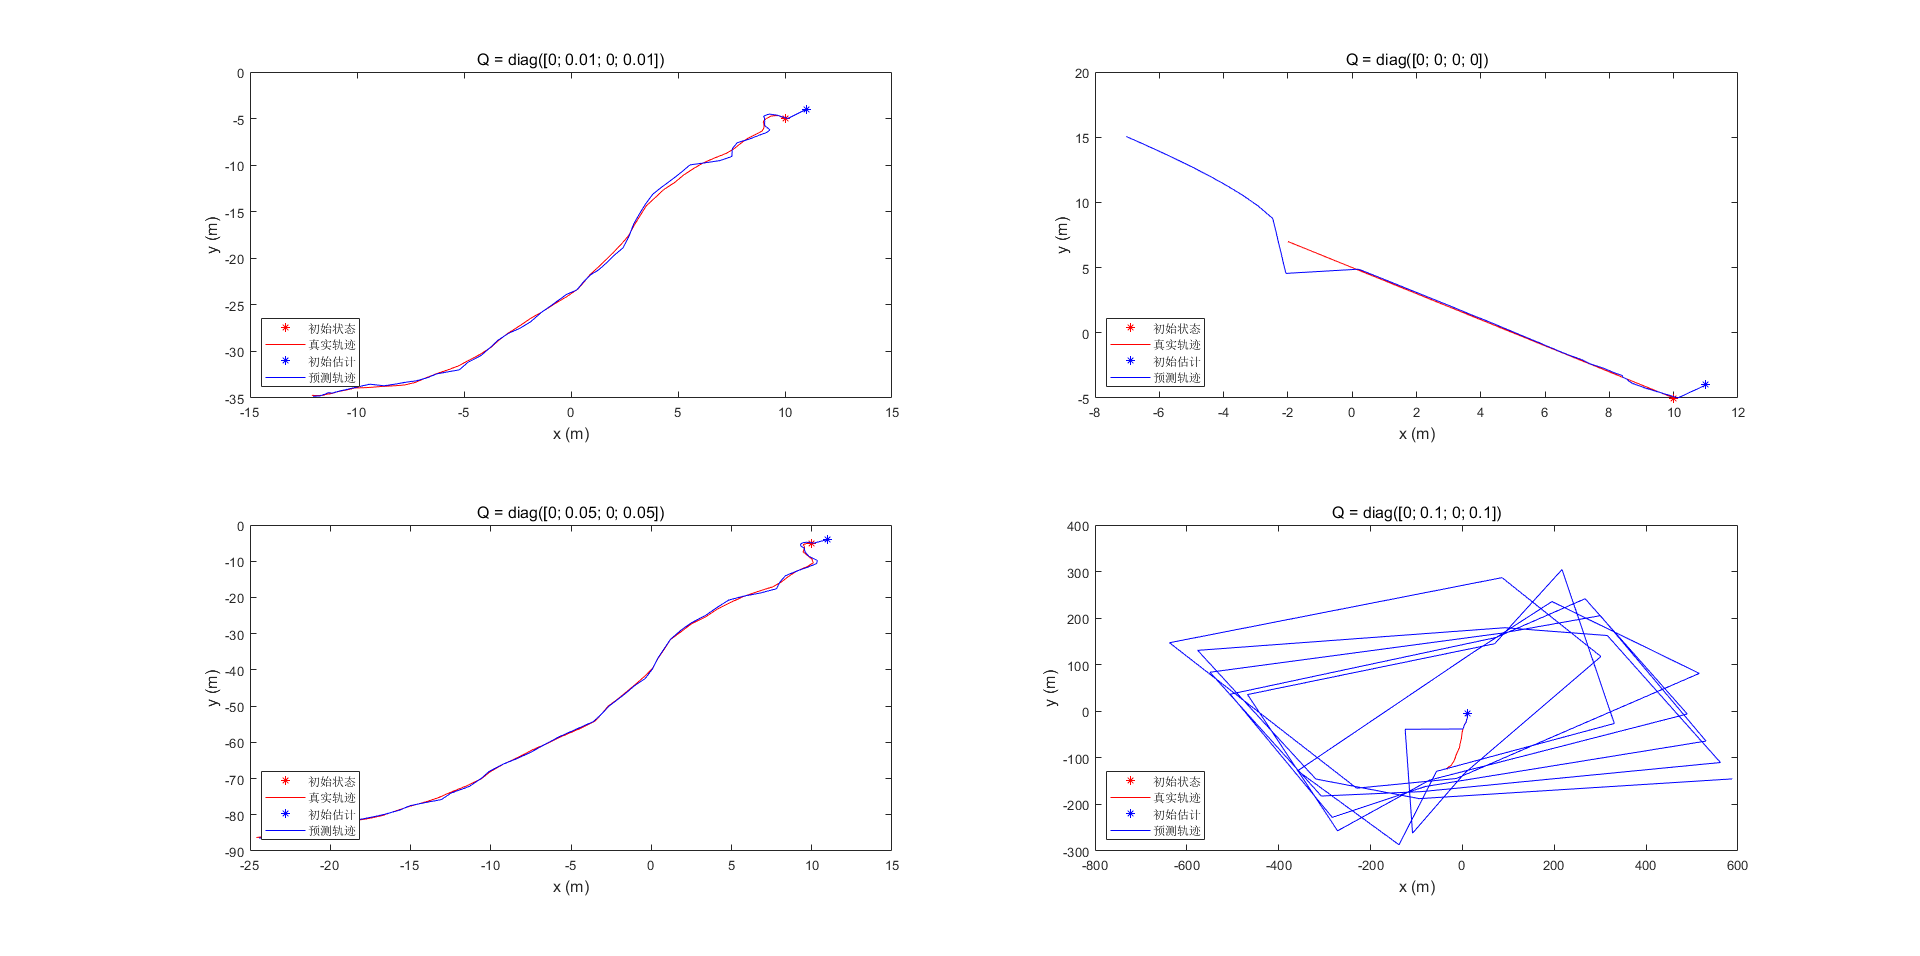
\includegraphics[width = 0.9\textwidth]{imgs/comp3.png}
    \caption{改变$\mathbf{Q}$}
    \label{fig:comp3}
\end{figure}

我们改变测量噪声协方差$\mathbf{R}$,发现其越小,预测越准确。其中,$\sigma_{\beta}^{2}$比$\sigma_{R}^{2}$敏感得多。
\begin{figure}[H]
    \centering
    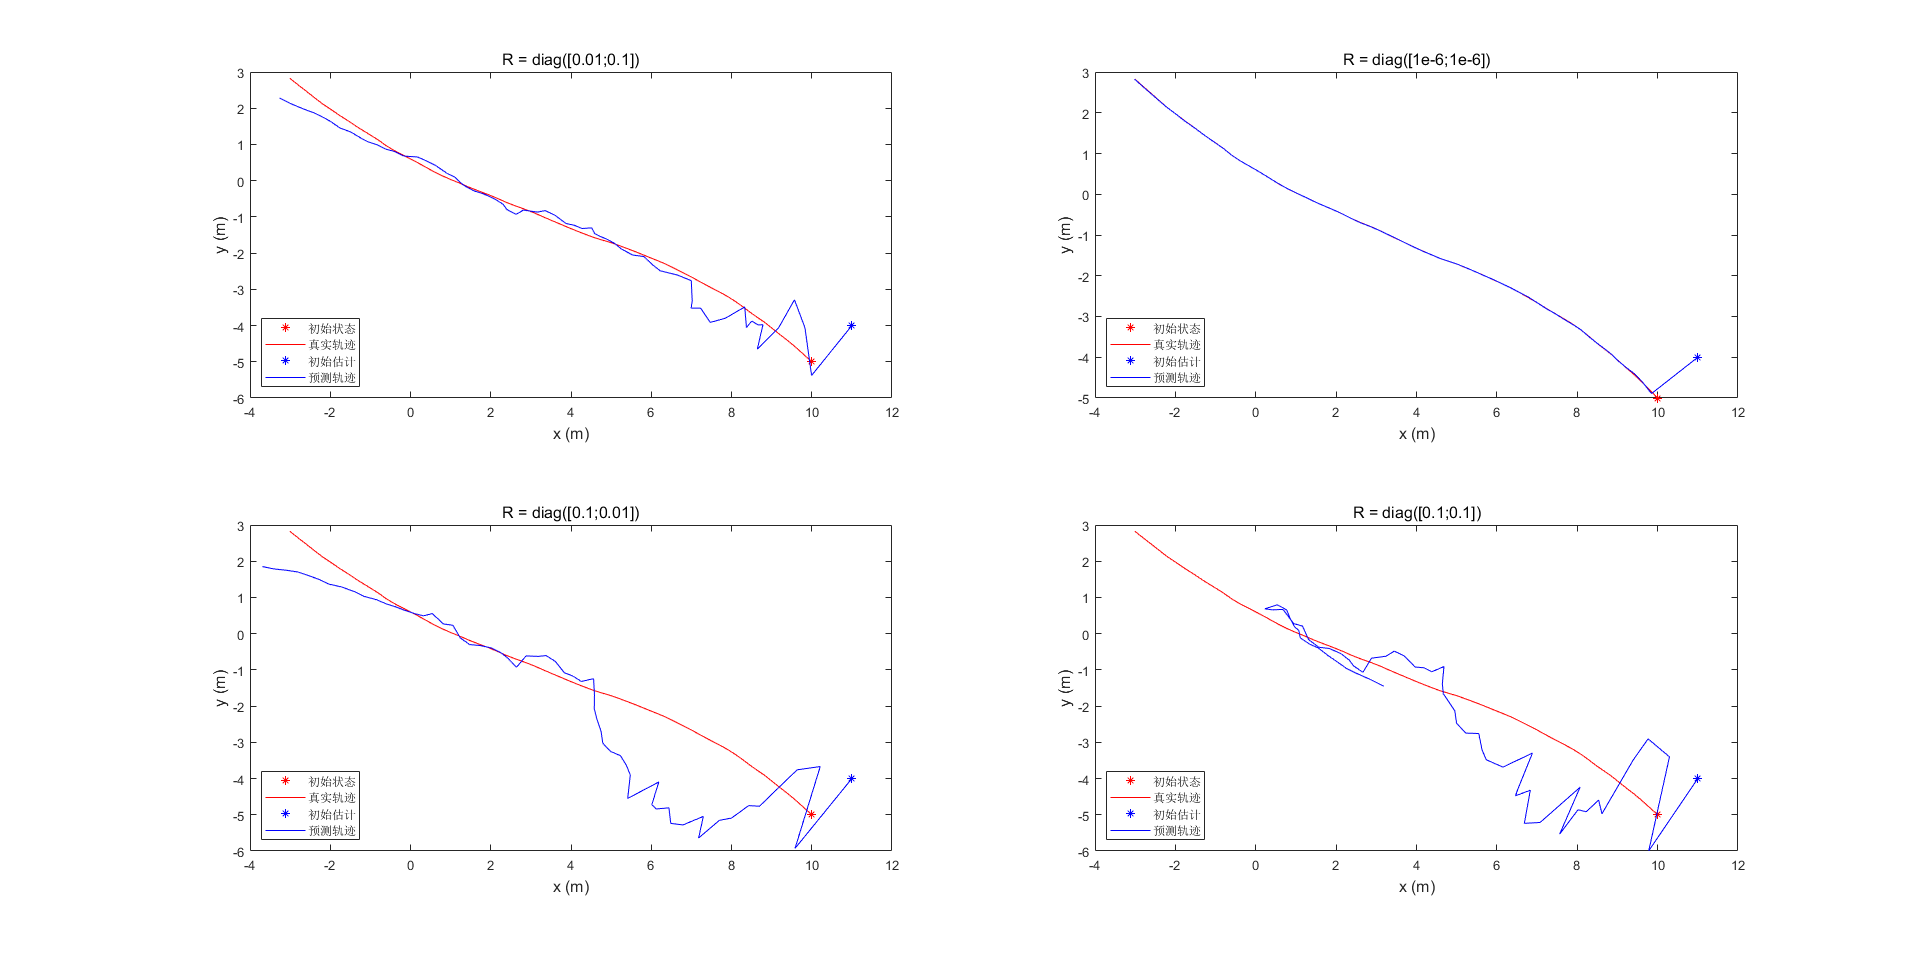
\includegraphics[width = 0.9\textwidth]{imgs/comp4.png}
    \caption{改变$\mathbf{R}$}
    \label{fig:comp4}
\end{figure}

%\newpage
\section{讨论与总结}

把算法中涉及到的状态转移方程和观测方程封装成了函数,便于修改参数、复用。在仿真实验中发现matlab内置的EKF函数自带对于雅可比矩阵的求解,无需自己设置,但是对于状态向量的格式有要求。

EKF虽然通过线性化能够对于非线性系统完成估计,但是当泰勒展开式的高阶项无法忽略时则会导致较大误差。而且现实中有很多函数很难求导出雅可比矩阵。而且想要求出雅可比矩阵就得先知道非线性函数的具体形式。

%\bibliography{ref}

\begin{refcontext}[sorting = none]
\printbibliography
\end{refcontext}
\end{document}
